\documentclass[../masters.tex]{subfiles}

\begin{document}
\graphicspath{{./imgs/}{../imgs/}} %look for images

\section{Hybrid Models}
In this section we generalise the graphical models of the previous sections as shown in Figure \ref{fig_hybridmod}. The variables retain their meaning as before but we again assume linearity of the models. The
use of switching stochastic variables $S$ allows for greater expressivity than before.     
\begin{figure}[H] 
\centering
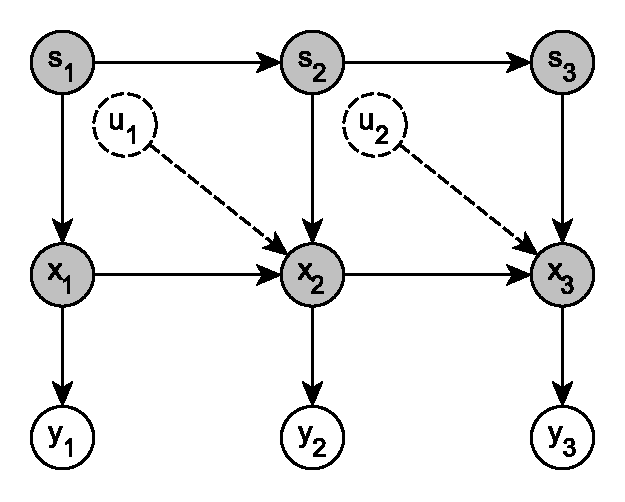
\includegraphics[scale=1.0]{hybrid_model.pdf}
\caption{Graphical model of this section}
\label{fig_hybridmod}
\end{figure}

Here is a picture where the reaction constant $k_0$ increases by an order of magnitude one second into the run. ``Nonlinear Model" = the actual system. ``Nonlinear model no switch" the state trajectory without the change in rate constant.
\begin{figure}[H] 
\centering
\includegraphics[scale=0.3]{temp.pdf}
\caption{Nonlinear switching}
\label{fig_hybridmod}
\end{figure}

Here is a picture of the linear switching reactor where both states are measured. As you can see it also closely follows the actual states (like the Kalman Filter when both states are measured). The difference is the switching model can change the model (or set of models) it uses for prediction (i.e. control) based on what it observes whereas the standard kalman filter only has one model... 
\begin{figure}[H] 
\centering
\includegraphics[scale=0.3]{temp2.pdf}
\caption{Linear switching}
\label{fig_hybridmod}
\end{figure}
Here we see relative contribution to the final state estimate of the 19 different models I used.
\begin{figure}[H] 
\centering
\includegraphics[scale=0.3]{temp3.pdf}
\caption{Nonlinear switching}
\label{fig_hybridmod}
\end{figure}


%\bibliographystyle{plain}
%\bibliography{research}

\end{document}